% Document type with options
\documentclass[fleqn,letterpaper,12pt]{report}

% Required packages and settings (DO NOT UPDATE THIS)
\usepackage{UN5390}
../LaTeXTemplates/Course/UN5390_Settings.tex

% Assignment-specific setting (UPDATE THIS WHEN NECESSARY)
\week{01}

% Document begins
\begin{document}

% Title (DO NOT UPDATE THIS)
\assignmenttitle

%
\phantomsection
\addcontentsline{toc}{section}{Problem \# 1}
\problem
Thinking of the Solution to that problem with the resources of that time, these are the some ways I think could improve the Hollerith’s technique.\newline
1). By Integrating the Pantograph and Card Reader. This can be done by having multiple pins to punch the card one for each value instead of just one pin to punch a hole and having the same mercury below that would enable the circuit to complete. The pins can be switched on or off. If the operator needs to punch holes for hole positions 5 in row 1 and 4 in row 2 etcetera he would turn the 4 pin in row 2 and 5 in row 1 and then punches in. The readings are noted in the dials. The punched cards can be kept for the records.\newline
2). By Integrating the individual dials associated with each value of all the machines which means if there are 10 card readers in the room, there would only be one dial for each value on the card. This could be done by analog Time Division Multiplexing using a commutator. So instead of noting individual machine dial counts, the main dial count associated with all the machines can be noted at the end of each session or so. The individual dials can be used for used to verify the count at the end of each session.\cite{Census}

The problem that I have always thought of in our current world that I think requires a radical new approach is the problem of electrical power generation. “Almost all electrical power on Earth is generated with a turbine,driven by wind, steam or burning gas.The turbine drives a generator”-Wikipedia.
Almost all new techniques we develop other than photovoltaic techniques or thermoelectric techniques which contribute very little to the demand, have at the end a turbine . If we could think of a radical, unconventional if not out of the box technique, maybe we could solve multiple problems associated with it such as Environmental and Depletion of resources and even Wars and global peace.\break
\newline
There are certain things which are noteworthy about the 1890 census apart from steep rise in the population.\newline
1. The increase in the number of questions for each family or farm from 26 to 30.\newline
2. The race question was not addressed as 'Colour' in the 1890 Census.



%
\newpage
\phantomsection
\addcontentsline{toc}{section}{Problem \# 2}
\problem
National Oceanic and Atmospheric Administration has nearly four-fold increase in computing capacity to innovate U.S forecasting in 2016 according to the website of the National Oceanic and Atmospheric Administration of the United States Department of Commerce. This investment is reportedly to advance the field of meteorology and improve global forecasts.

The Computers are called Luna and Surge located at computing centres in Reston, Virginia and Orlando, Florida. The total operational capacity of these new computers rests around 5.78 petaflops after the upgrade contract with IBM.\cite{latest}

The Upgrades reportedly will now enable the two operational Supercomputers to run The Global Weather Forecast system(GFS) with greater resolution that extends further out in time. The new GFS will increase resolution from 27km to 13km out to 10 days and 55km to 33km from 11 to 16 days. In addition, the Global Ensemble Forecast System(GEFS) will be upgraded by increasing the number of vertical levels from 42 to 64 and increasing the horizontal resolution from 55km to 27km out to 8 days and 70km to 33km from 9 to 16 days. 


In the words of Louis Uccellini Ph.D., director, NOAA’s National Weather Service. “"By Increasing our overall capacity, we’ll be able to process quadrillions of calculations per second that all feed into our forecasts and predictions. This boost in processing power is essential as we work to improve our numerical prediction models for more accurate and consistent forecasts required to build a Weather Ready Nation."”\cite{NOAA}

In Summary, this increase in supercomputing strength will allow NOAA to upgrade many operational models such as:

1).Upgrade the High Resolution Rapid Refresh Model(HRRR) will help meteorologists predict the amount, timing and type of precipitation in winter storms and timing location and structure severe thunderstorms as reported by the NOAA website.

2). Implementation of the Weather Research and Forecasting Hydrologic Modeling System (WRF-Hydro) will expand the national Weather Service’s current water quantity will enhance the forecasts of flow.soil moisture , snow water equivalent, evapotranspiration, runoff and other parameters for 2.67 million river and stream locations across the country which is a 700-fold increase in the spatial density. This helps enable forecasters to more accurately predict droughts and floods.

3).The Hurricane Weather Research and Forecasting Hydrologic Modeling System(WRF-Hydro) will enable connection between factors such as air, ocean and waves to improve forecasts of hurricane tracks and intensity.
%
\newpage
\phantomsection
\addcontentsline{toc}{section}{Problem \# 3}
\problem
The Collaboration of Oak Ridge, Argonne, and LiverMore(CORAL) is a joint procurement activity among three of the Department of Energy’s National Laboratories laughed in 2014 to build state of the art high performance computing technologies. CORAL is jointly led by the Office of Science’s too Leadership Computing Facility centres at Oak Ridge National Laboratory(ORNL) and Argonne  National Laboratory (ANL) and the National Nuclear Security Administration’s facility at Lawrence Livermore National Laboratory(LNL). These state of the art Computing technologies are essential for supporting US national nuclear security and are key tools used for technology advancement and scientific discovery.

High Performance Computing(HPC) technologies procured under this announcement deliver both much greater capabilities and energy efficiency. The aim to to procure technologies that deliver 20-40x the capabilities of todays’s computers with a similar size and power footprint. The applications of these high performance computing technologies are wide and include \newline
1).Assuring the viability of US nuclear deterrent and supporting US policy in counter terrorism.\newline
2).Discovering and designing new materials.\newline
3).In advanced fields including astrobiology, biology, chemistry and other fields.\newline
4).Economic competitiveness and Scientific Discovery.\newline
5).Sustained Technical Leadership.

The three CORAL labs developed a single request for Proposal(RFP) that specified the requirements and desired features of a system to meet the needs of Department of Energy’s Office of Science and National Nuclear Security Administration. One requirement was that the ORNL and ANL would have computers with different architectures to manage risk. Secretary Moniz announced \$325 million to build two state-of-the-art supercomputers at the Department of Energy’s Oak Ridge and Lawrence Livermore National Laboratories.\cite{ORL}

DOE’s Office of Science and National Nuclear Security Administration signed a Memorandum of Understanding to increase coordination in high performance computing research and development and HPC acquisitions.The CORAL request for proposal was released in January 6,2014 and proposals were received on February 18,2014. The proposals were evaluated and two different computer architectures were selected by the three laboratories.\cite{DOE} \cite{IBM}

Technical Details: \newline
Both CORAL award’s announced IBM Power Architecture, NVIDIA’s Volta GPU and Mellanox’s Interconnected technologies to advance key research initiatives. Oakridge’s new system Summit, is expected to perform atleast five times the present system Titan. Livermore’s new supercomputer,Sierra, is expected to perform atlas seven times faster than the present current LLNL’s Sequia.
Argonne is yet to announce its CORAL award.
\newpage
Specifications:\cite{Sierra}\newline
The specifications for both Summit and Sierra are as follows: \newline
1). IBM POWER processors and NVIDIA Volta GPUs \newline
2). Mellanox InfiniBand InterConnection Network \newline
3). IBM Elastic Storage \newline
4). Maximum Projected power envelope of 10 MW 

NVLINK: \newline
The GPUs in Titan are connected today to the CPUs through a PCI Express (PCIe) interface, which limits how fast the GPU’s can access the CPU memory system. Summit will have a new high-bandwidth interconnect from NVIDIA, called NVLINK, and it will improve accelerated software application performance. With NVLink, the data moves between the CPU memory and GPU memory 5-12 times faster than PCIe, making GPU-accelerated applications run much faster on Summit. 

Unified Memory Feature: \newline
The faster data movement that comes with the NVLink, coupled with another feature known as Unified Memory, will simplify GPU accelerator programming. Unified Memory allows the programmer to treat the CPU and GPU memories as one block of memory. The programmer can operate on the data without worrying about whether it resides in the CPU’s or GPU’s memory.

Compilers: \newline
PGI, GCC, XL, LLVM 

Performance Tools: \newline
VAMPIR, TAU, HPC Toolkit (IBM), nvprof, gprof, Open|SpeedShop, and HPCToolkit (Rice) 

Debugging Tools: \newline
DDT, cuda-gdb, cuda-memcheck, Valgrind, stack trace analysis tool (STAT), pdb.

Power Consumption: \newline
10 MW or less which is 10% higher than the present Titan. 

User Access: \newline
Anticipated to be in the calendar year of 2018 \newline 


\vfill

%
\newpage
\phantomsection
\addcontentsline{toc}{section}{Problem \# 3}
\problem
MATLAB is short for Matrix Laboratory developed by MathWorks.  It is a multi-paradigm computing environment. It supports both Imperative and Object Oriented Programming. It was first developed by Cleve Moler , the then chairman of Computer Science at the University of New Mexico. Later was commercialised by Jack Little and Steve Bangert along with Cleve Moler founding MathWorks. 

Basics:\newline
The default screen when MATLAB is started consists of three panels:
Current Folder — Access your files. 
Command WIndow — Enter commands at the command line, indicated by the prompt (/>/>).,
Workspace— Explore data that you create or import from files

Keywords:\newline
To verify is a word is a keyword in MATLAB, we can use “iskeyword” function.\newline
These are the list of most common MATLAB keywords:\newline
	'break'\newline
    'case'\newline
    'catch'\newline
    'classdef'\newline
    'continue'\newline
    'else'\newline
    'elseif'\newline
    'end'\newline
    'for'\newline
    'function'\newline
    'global'\newline
    'if'\newline
    'otherwise'\newline
    'parfor'\newline
    'persistent'\newline
    'return'\newline
    'spmd'\newline
    'switch'\newline
    'try'\newline
    'while'
	
Variables\newline
There are several different data types in MATLAB . We do not have to specify the data type when declaring a variable in MATLAB. 
The different data types are listed below:\newline
1.Floating Point Numbers: \newline
Class: Single, Double\newline
Floating Point Number is the default data type in MATLAB. They are used to store real numbers. e.g. F = 1.89938532. \newline
2.Integers: Integers are of the following classes in MATLAB.  
Class: uint8, int8, uint16, int16, uint32, int32, uint64 and int64.\newline
This data type is more memory efficient and allows for storage of whole numbers. "u" stands for unsigned integers while "8,16,32,64" stand for the number of bits for storage. e.g. C = uint16(256) \newline
3. Characters and Strings:Used to store text. \newline
Class: char \newline
A string is an array of characters while char signifies each one. e.g. c = “Hello” \newline
4.Boolean: \newline
class: logical \newline
Used to Store true(1) or false(0) \newline
5.Structures: \newline
Class: Struct \newline
Used to Store varying lengths of Data types. the data types are accessed using an index.

Matlab is an interpreted language meaning it is dynamically compiled. It allows numerical calculations and the Visualisation of the results associated with it.

The programming environment is called Command Window and the variables associated with the program are stored in the Workspace. These variables can be checked out by the command ‘who’
‘clc’ clears out the Output of the command window. ‘clear’ clears out all the variables stored in the workspace.

The key thing about MATLAB is that all data in variables are realised as double precision array. Hence the name, Matrix Laboratory.

Files:\newline
MATLAB stores data to *.mat files by default in the default path.”save” enables one to save the files.\newline
uisave - includes user interface.\newline
hgsave -saves figures to files *.fig by default
diary[filename]- All text input in the command window to a text file. This is equivalent to directing a output to a file in linux shells.

Files can be loaded by using the “”load [filename.ext]”” in MATLAB. 
There are functions that enable generic import of data.
import data examines the extension and loads the data depending on the extension.\newline
'uiimport' opens a window to examine data

Functions:\newline
MATLAB supports anonymous function creation from the command line.\newline
General functions can also be written in MATLAB with the use of the keyword “"function"”
\newpage
Complex Numbers:\newline
MATLAB supports complex numbers and also supports visualisation of complex functions. a complex number can be declared as:\newline
comp = 1+1i;

Arrays:\newline
Arrays are indexed using Integers. The first Array Element is indexed with a '1' instead of a '0' contrary to most programming languages maybe because MATLAB was developed using FORTRAN and FORTRAN used this convention.

Visualisations:\cite{MATLAB}\newline
MATLAB supports visualisations in 2D and 3D.\newline
The most common visualisations are:\newline
1.Plot : Renders a 2D line in Cartesian Coordinate System. e.g. plot(x,fx)\newline
2.Polar Plot: Renders a plot using θ and r(θ). e.g.\newline polar(t,sin(2*t))\newline
3.3D Plot: plot3(l,f,d);grid on;\newline
4. Contours: Enables visualisation of vectors. e.g. contour(x,y,x)
5.Mesh: Creates 3d lot using Vectors x and y and a matrix z that have the same number of elements. e.g mesh(x,y,z). MATLAB also supports annotations of the visualisations.

Scripts:\newline
There are two types of m-files:\newline
scripts and Functions:\newline
The key difference being that general scripts run using present variables in the workspace. Functions on the other hand wholly contain themselves.They possess their own workspace keeping workspaces separate from the current workspace. also limiting the scope of the variables.

Control Flow:\newline
MATLAB’s control statements are similar to the control statements in most languages. There are the \newline
1. if and elseif statements.\newline
e.g\newline
if expression\newline
	statements\newline
else if expression2\newline
	statements\newline
end

2. The common switch statement:
switch variable\newline
case variable1:\newline
	statements\newline
case variable2:\newline
	statements\newline
end

3. There is also a provision for exceptions
e.g\newline
try \newline
	statements\newline
catch\newline
	statements\newline
end

4. The FOR loop and the WHILE LOOP and BREAK, CONTINUE and RETURN statements.

Built in Mathematical Functions:\newline
MATLAB gives many built in functions to solve everyday numerical problems. Since Matlab realises all data as matrices, the data is processed using most common matrices operations such as Transpose and built in functions to solve higher order differential equations both ordinary and partial.

Git Support:\newline
MATLAB also supports Git Source control. 

I/O Operations:\newline
MATLAB also supports many I/O operations such as reading and writing from files. Socket programming and writing to a USB port.
The process for reading from or writing to  file is similar to other programming languages
/>/>fid = fopen(‘myfile.txt’,’r) %  open file to read/write or both
/>/>spec = fscanf(“Hello”) %scanf file for Hello and manipulate as required.
/>/>fclose(fid) %closes file with id

OOP/’s\newline
Like discussed in the beginning, MATLAB supports multiple programming paradigms. Although MATLAB supports object oriented programming, technically MATLAB is not a fully Object Oriented Programming Language.
It supports Polymorphism, Inheritance and Encapsulation.

Toolboxes:\newline
The most important thing about MATLAB is that MATLAB offers various toolboxes such as the Image processing Toolbox, the Signal Processing toolbox, Optimisation toolbox etc. It also supports parallel programming and algorithms that can be run on supported hardware.

\vfill

%
\newpage
\phantomsection
\addcontentsline{toc}{section}{Problem \# 3}
\problem
This famous Approximation of Pi is one of the findings by the popular Indian Mathematician Srinivasa Ramanujan which computes a further eight decimal places of Pi with each summation term in the series. These approximations later lead to Ramanujan-Sato series where these converging series for approximating Pi are generalised.\newline
The MATLAB Program file for calculating the error in this approximation is in the file "pi\_sr.m" in the folder "un5390\_f2016\_slanka/CourseWork/Week\_01/slanka\_01"\cite{Pi} 
\begin{figure}[ht!]
\centering
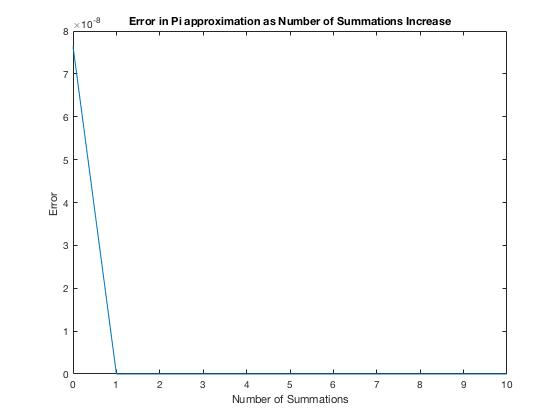
\includegraphics[width=140mm]{Pi_sr.jpg}
\caption{Error vs Number of Summation elements\label{overflow}}
\end{figure}


\vfill

%
\newpage
\phantomsection
\addcontentsline{toc}{section}{Problem \# 3}
\problem
The bash shell script for the Conversion of seconds into Human readable 
Hours:Minutes:Seconds format is in the file "seconds2hms.sh" in the directory "un5390\_f2016\_slanka/CourseWork/Week\_01/slanka\_01" of the MichiganTech Repository.\cite{tc}
\vfill
\newpage

%
\newpage
\phantomsection
\addcontentsline{toc}{section}{Problem \# 3}
\problem
The bash shell script for the Conversion of Julian Year and days into general Calender date 
Year-Month=Day format is in the file "julian2ymd.sh" in the directory "un5390\_f2016\_slanka/CourseWork/Week\_01/slanka\_01" of the MichiganTech Repository.\cite{tc}
\vfill
\newpage
% References
% http://tex.stackexchange.com/questions/84099/bibliographies-from-multiple-bib-files
\phantomsection
\addcontentsline{toc}{section}{References}
\section*{References}
\bibliographystyle{unsrt}
\bibliography{sgowtham,slanka} % REPLACE john WITH YOUR MICHIGAN TECH ISO USERNAME

% Document ends
\end{document}